 \addtolength\abovedisplayskip{-1\baselineskip}%
  \addtolength\belowdisplayskip{-1\baselineskip}%
  
\begin{tikzpicture}
\node[] (data) {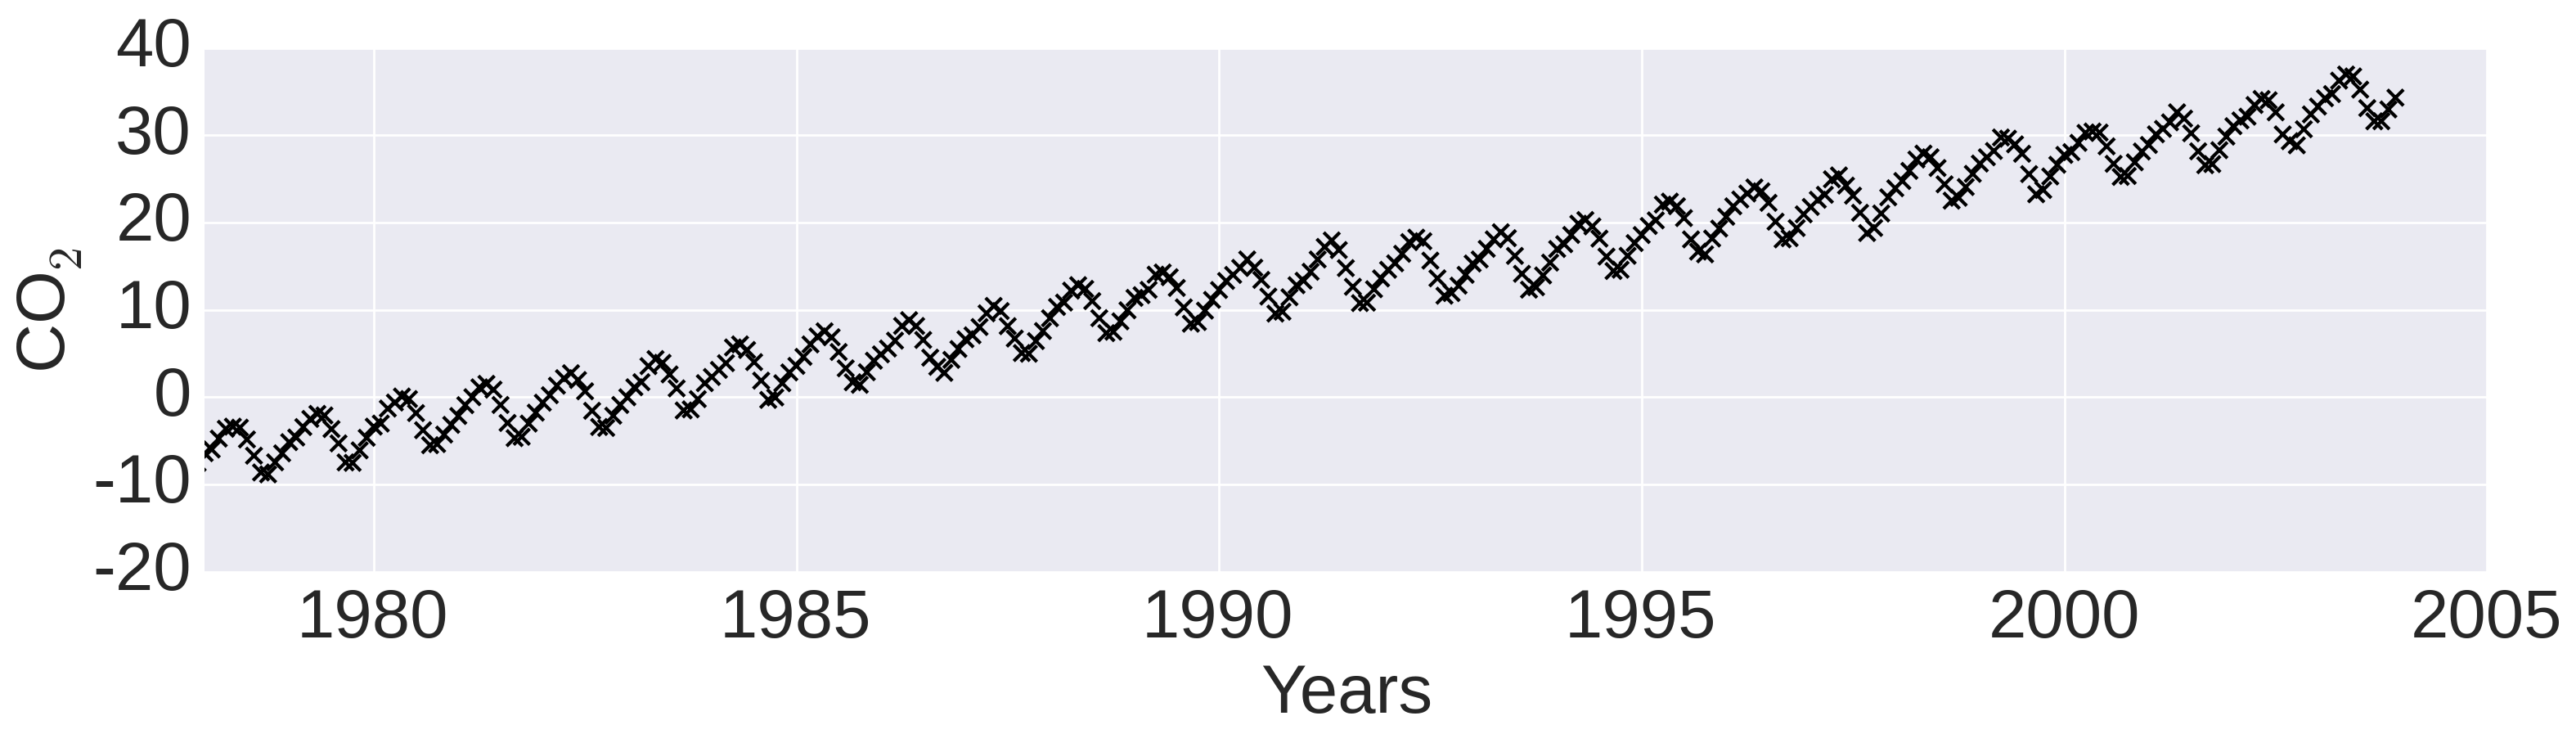
\includegraphics[width=0.7\textwidth]{figs/mauna_data.png}};
\node[below = 2cm of data] (post_param_helper) {};
\node[above = 1cm of post_param_helper] (post_param_helper_1) {};
\node[below = 1cm of post_param_helper] (post_param_helper_2) {};
\node[left = -2cm of post_param_helper] (post_param) {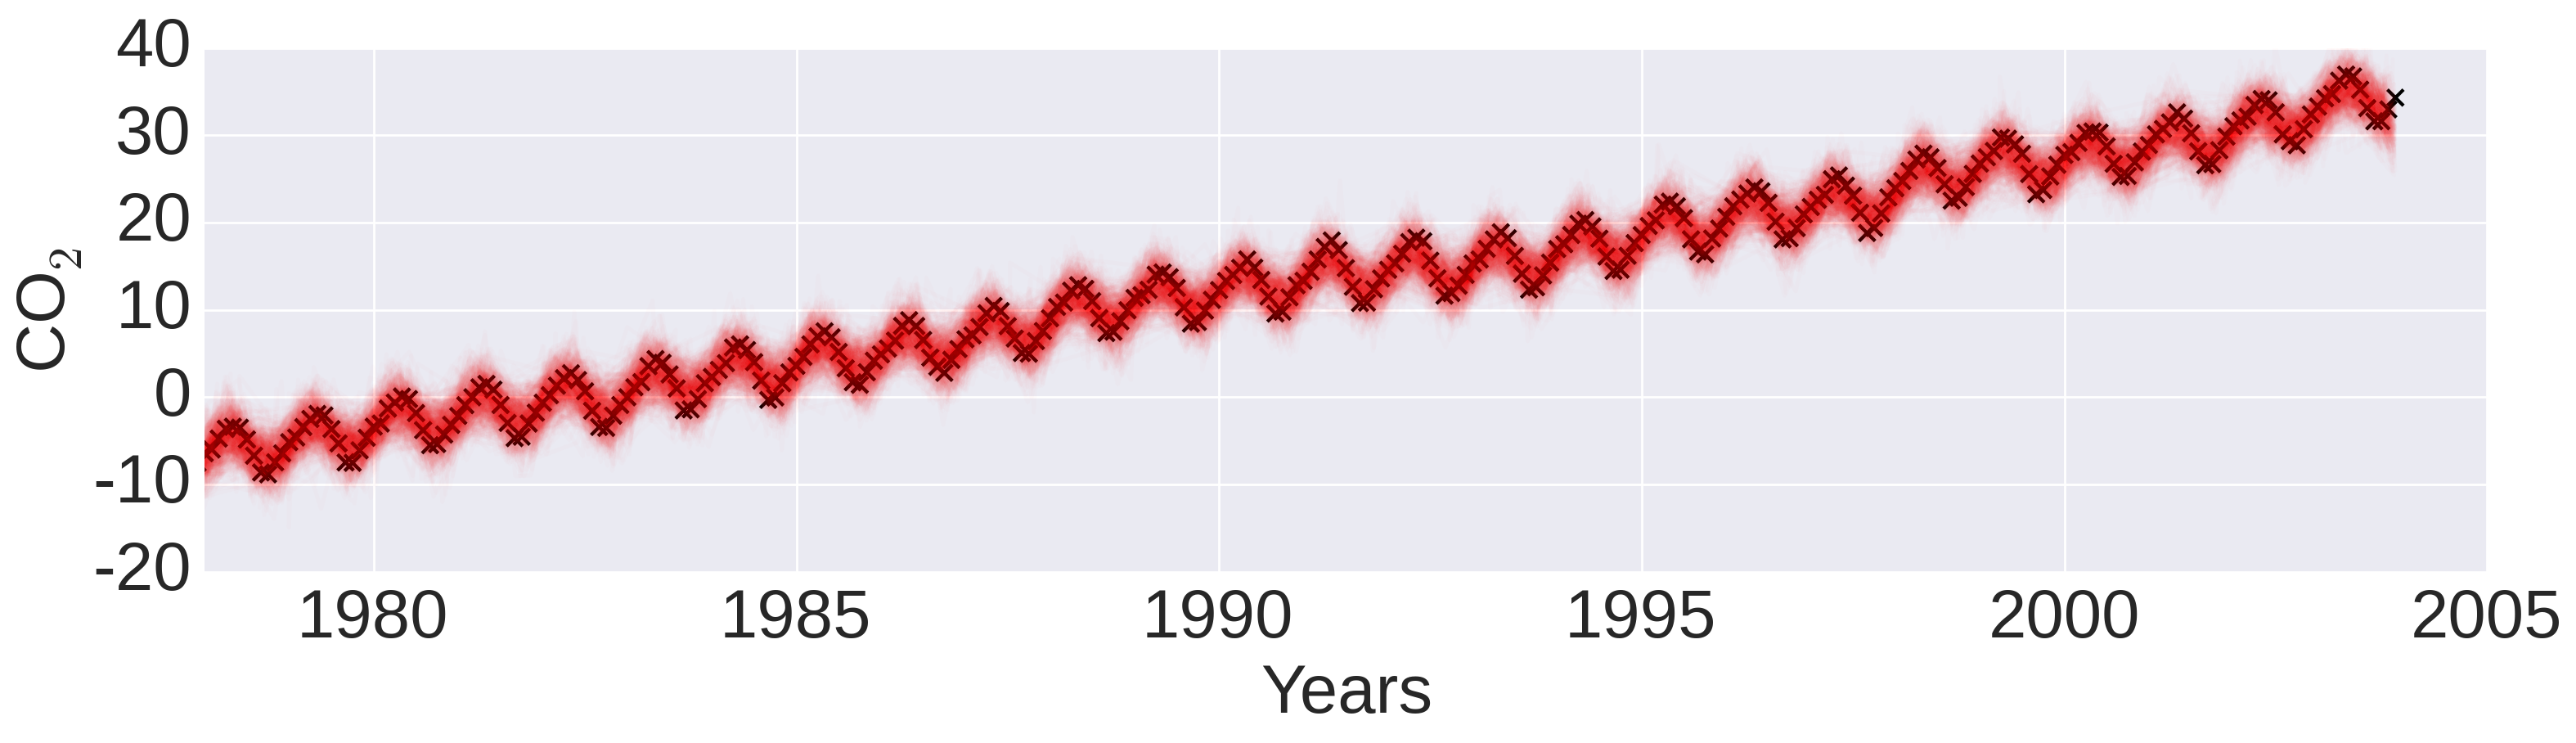
\includegraphics[width=0.6\textwidth]{figs/mauna_sample_1.png}};
\node[draw,rectangle,color=red,dashed,right = 2cm of post_param_helper,yshift=0.5cm] (zoom) {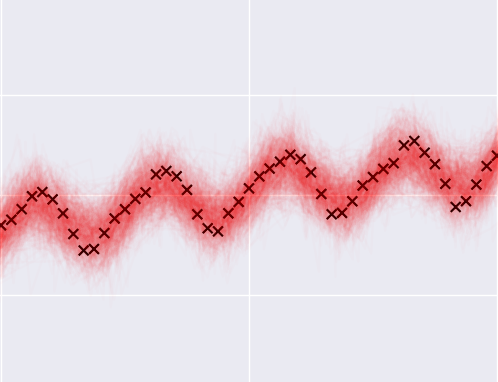
\includegraphics[width=0.3\textwidth]{figs/mauna_zoom.png}};
\node[draw,rectangle,color=red,dashed,left = 2.8cm of zoom, minimum width = 1.5cm, minimum height = 1.2cm] (zoom_in) {};
\node[below = 0.7cm of post_param_helper_2] (posterior) {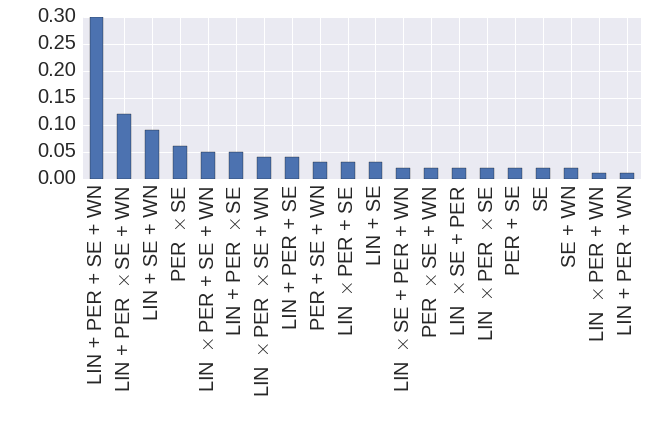
\includegraphics[width=0.7\textwidth]{figs/mauna_structure.png}};

\node[draw,rectangle,below = 0.7cm of posterior] (formula) {\color{black}
$\mathbf{K}=\text{LIN} + \text{PER} + \text{SE} + \text{WN}$};
\node[draw,rectangle,below = 0.7cm of formula] (formula_param_1) {\color{black}
$= 2.7^2(x x^\prime) + 5.6^2 \exp \bigg( \frac{2 \sin^2 ( \pi (x - x^\prime)/3.7}{6.4^2} \bigg)
+ 0.4^2 \exp(-\frac{(x-x^\prime)^2}{2 \times 6.3^2}) +  1.9^2 \delta_{x,x^\prime} \label{eq:WN}$ };


\node[draw,rectangle,below = 0.7cm of formula_param_1,text width = \textwidth,minimum height = 1.5cm] (paragraph){\color{black}\footnotesize {\bf Qualitative Interpretation}:
The posterior peaks at a kernel structure with four additive components. Additive components hold globally, that is there are no higher level, qualitative aspects of the data that vary with the input space. The additive components are as follows: (i) a linearly increasing function or trend; (ii) a periodic function; (iii) a smooth function; and (iv) white noise.};







\node[draw, rectangle, left = -1.755cm of posterior,minimum width = 0.45cm, minimum height = 5.8cm,yshift=0.2cm] (mark_structure) {};
%\node[draw,very thick, rectangle, below = 1.1cm of data,minimum width = \textwidth, minimum height = 15cm] (posterior_frame) {};

%\node[left = 1.3cm of mark_structure] (paragraph_helper){};
\node[below =0.6cm of mark_structure,inner sep = 0pt,outer sep=0pt] (formula_helper) {};
\node[above =0.7cm of formula,inner sep = 0pt,outer sep=0pt] (formula_helper_2) {};

%\draw[-,dashed] (mark_structure.south) -- (formula_helper);
%\draw[-,dashed] (formula_helper) -- (formula_helper_2);
%\draw[->,dashed] (mark_structure) -- (paragraph_helper);
%\draw[->,dashed] (formula_helper_2) -- (formula);

\draw[->] (data) -- (post_param_helper_1);
\draw[->] (post_param_helper_2) -- (posterior);
\draw[->] (formula_helper_2) -- (formula);
\draw[-] (mark_structure) -- (formula_helper);
\draw[-] (formula_helper) -- (formula_helper_2);
\draw[->] (formula) -- (formula_param_1);
\draw[->] (formula_param_1) -- (paragraph);

\draw[->,dashed,red] (zoom_in) -- (zoom);

%\draw[->,line width=1pt,double distance=2pt] (data) -- (post_param);
\end{tikzpicture}
\addtolength\abovedisplayskip{1\baselineskip}%
\addtolength\belowdisplayskip{1\baselineskip}%


